\documentclass{article}
\usepackage{color} 
\usepackage{tikz} 
\usetikzlibrary{babel ,scopes ,intersections ,calc ,bending ,positioning ,quotes ,graphs ,fadings ,decorations ,angles ,automata ,babel ,backgrounds ,calc ,calendar ,chains ,circuits ,er ,external ,external ,external ,fadings ,fadings ,external ,fadings ,fit ,fixedpointarithmetic ,fpu ,lindenmayersystems ,math ,matrix ,mindmap ,folding ,patterns ,petri ,plothandlers ,plotmarks ,profiler ,shadings ,shadows ,spy ,topaths ,through ,trees ,turtle ,datavisualization ,intersections ,curvilinear}

\begin{document}
\pagenumbering{gobble}
    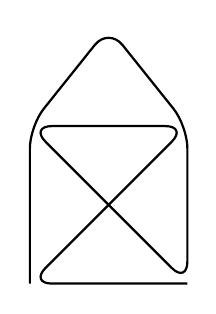
\begin{tikzpicture}
        \tikz \draw[thick,rounded corners=8pt]
(0,0) -- (0,2) -- (1,3.25) -- (2,2) -- (2,0) -- (0,2) -- (2,2) -- (0,0) -- (2,0); 
    \end{tikzpicture}
\end{document}
